Today, private communication is protected by cryptographic systems that rely on the hardness of specific number-theoretic problems. The link between the two disciplines, cryptography and number theory, first established in the revolutionizing work of Diffie and Hellman \cite{DH76} and later reinforced by the work of Rivest, Shamir, and Adleman on RSA \cite{RSA78}, has led to extremely efficient ways to exchange information privately. The effect of these discoveries on our everyday life is enormous as we can hardly imagine ourselves being unable to buy goods, make reservations or handle other types of financial operations over the Internet.  

The elegance of number-theoretic constructions has been shadowed by arguably the most famous quantum algorithm -- the period-finding algorithm by Shor \cite{Shor97}, first appeared in 1996. Provided a large-scale quantum computer is built, all the cryptographically relevant number-theoretic problems, like integer factorization or the discrete logarithm problem, can be efficiently solved by Shor's algorithm. The existence of such a quantum computer may look unrealistic today as there are several serious obstacles on the way to build a quantum device that could be of any threat to our modern cryptosystems; yet many concerns have been raised on the security of the deployed systems. These worries are also backed up by the progress in classical methods for factoring large numbers and solving the discrete logarithm problem in multiplicative groups of finite fields. For example, the general number field sieve algorithm, the most efficient algorithm known for factoring large integers, allows to factor $N$ in time $L_N(1/3, 1.902)$-- a function\footnote{where $L_N$ is defined as $L_N(\alpha, c) = \exp{(c+\smallo(1) (\log N )^{\alpha} (\log \log N)^{1-\alpha}}$}  truly sub-exponential in the bit-length of $N$.

Hard problems on a lattice in $\R^n$ offer an attractive alternative to the aforementioned number-theoretic problems and serve as a foundation to what is now known as \emph{lattice-based cryptography}. 


\begin{figure}[h]
	%\centering
	%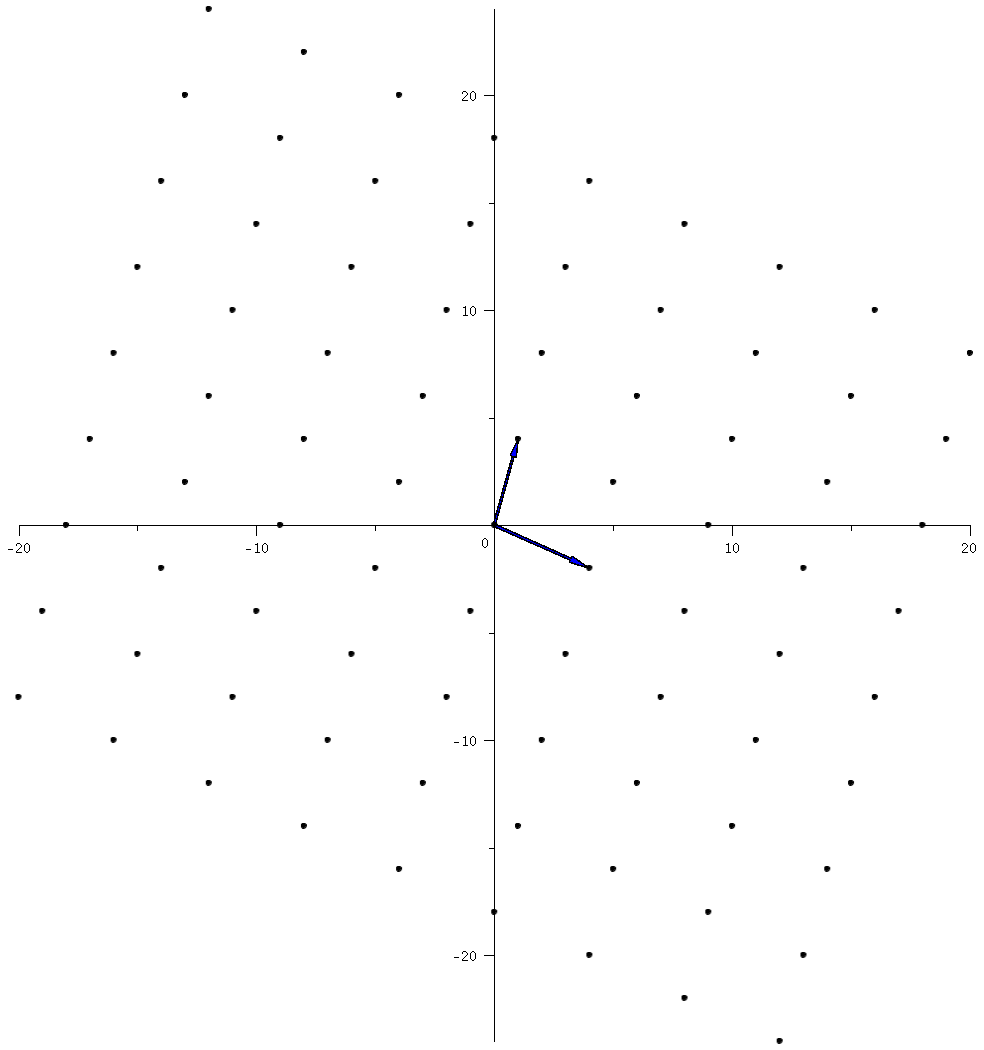
\includegraphics[trim={3cm 7cm 3cm 7cm}, clip, scale=0.2]{../2dLattice}
	\centering
	%\raisebox{0pt}[60pt][100pt]{
	%\framebox(60,100){
					\begin{tikzpicture}[framed,background rectangle]
						\begin{scope}
						\clip (-100pt,-60pt) rectangle (110pt, 100pt);
						\foreach \y in {-5,...,5}
						\foreach \x in {-5,...,5}
							\filldraw(\x*40pt+\y*10pt, 10pt*\x+20pt*\y) circle (1pt);
							\filldraw(0pt,0pt) circle (1pt) node[below]{ $0$};
						
						\draw[->, -stealth, black, shorten >=1pt] (0,0) -- (50pt, 30pt) node[font=\scriptsize, below, xshift=1pt]{$\bvec_1$};
						\draw[->, black, -stealth, shorten >=1pt] (0,0) -- (60pt, 50pt) node[font=\scriptsize, below, xshift=1pt]{$\bvec_2$};
						
						\draw[->, thick, -stealth, shorten >=1pt] (0, 0) -- (10pt, 20pt) node[font=\scriptsize, left]{$\vvec$};
						\end{scope}
					\end{tikzpicture}
	%}
	\caption[2-dim.\ lattice]{2-dimensional lattice with a basis $\{\bvec_1, \bvec_2\}$. $\vvec$ is one of the shortest vectors of this lattice.}
	\label{fig:2dLattice}
\end{figure}

A lattice is a set of points in $\R^n$ where each point is an integer linear combination of $n$-linearly independent vectors $\bvec_1, \ldots, \bvec_n \in \R^n$ known as a lattice-basis. An example of a 2-dimensional lattice with a basis is shown in Figure~\ref{fig:2dLattice}.

Lattices have attracted the attention of mathematicians since the late 18$\th$ century. Early works of Gauss and Lagrange aimed at finding short lattice bases in $\R^2$ have evolved into a whole range of algorithms known as lattice-basis reduction algorithms. The publication of \emph{Geometrie der Zahlen} by Hermann Minkowski at the beginning of the previous century marks the birth of the Geometry of Numbers -- a branch of number theory that studies convex bodies and lattice points contained in these bodies. 

In more recent time, lattices have become an active research topic in various computer science areas like integer programming \cite{Lenstra83}, complexity theory \cite{STOC:GolGol98, FOCS:Khot03}, and many others. Cryptography finds itself among this list as well. Interestingly, lattices stepped into cryptography as a destructive tool: Coppersmith's method to find small roots of low-degree polynomials \cite{Cop01}, an algorithm of Lagarias-Odlyzko for the low-density subset-sum problem \cite{LO86}, rounding techniques for the hidden number problem \cite{SODA:BonVen97} -- all these methods form an incomplete list of cryptanalytic tools based on lattices.

It was in 1996 when Ajtai shows in his celebrated paper \cite{STOC:Ajtai96} how to \emph{construct} cryptographic primitives from lattices. Ajtai's breakthrough is acknowledged as the starting point of the lattice-based cryptography that has been flourishing over the last 20 years.

Another significant milestone in the lattice-based cryptography era is the work of Regev \emph{On Lattices, Learning with Errors, Random Linear Codes, and Cryptography} \cite{STOC:Regev05}. While Ajtai's discovery allows to construct primitives that emerge from one-way functions such as collision-resistant hash functions and signatures, the question of building a public key cryptosystem remained open. Regev was the first to present a public key cryptosystem and relate its hardness to the problem of finding short vectors in a lattice known as the Shortest Vector Problem (\SVP) (see Figure~\ref{fig:2dLattice}).

The conjectured security against quantum attacks is one among several other attractive features of lattice-based constructions. Not only does Ajtai show how to build a primitive, he also proves that this primitive is hard to break unless \emph{all} instances of a certain lattice-problem are easy to solve. This connection is known as the \emph{worst-case} hardness. What it means is that a random instance of a problem (which, in a cryptographic setting, translates into a randomly chosen key-pair of a user) is as hard as the worst-case instance of this problem. Such a remarkable feature is not shared by number-theoretic problems like RSA: for instance, some large numbers are easier to factor than others. 

More importantly from a practical side, lattice-based cryptosystems are very efficient and highly parallelizable. Typical computations involve linear operations on matrices modulo a small integer. Primitives based on special \emph{ideal} lattices reduce the communication overhead thus making the constructions truly competitive with their number-theoretic counterparts.

Despite all these nice features, lattice-based cryptography is not yet widely deployed\footnote{In July 2016, Google has announced \cite{Google} that they incorporated a lattice-based public key-exchange scheme \emph{The New Hope} \cite{NewHope} for experimental purposes.}. Leaving aside costs of setting up a new algorithm into a communication channel, we still have theoretical questions to be answered before we could let lattice-based cryptography drive the real-world private communications. 

These questions are primarily of cryptanalytic nature. How hard are the lattice-problems underlying a cryptosystem? In particular, what are the best algorithms for the Shortest Vector problem? In this thesis, we address these questions.

The dissertation consists of two parts. The first part analyzes the complexity of the problem that underlies all known lattice-based cryptosystems. The second part is devoted to the Shortest Vector Problem. We now detail on each part.
\vspace{7pt}
\begin{center}
	\textbf{Part I. Learning with Errors as Bounded Distance Decoding}
\end{center} 
The cryptosystem of Regev presented in \cite{STOC:Regev05} does not \emph{directly} rely on a lattice-problem. It relies instead on the so-called \emph{Learning with Errors} problem. In \cite{STOC:Regev05}, Learning with Errors (\LWE), an average-case hard problem, is proved to be at least as hard as a certain problem on lattices. This result enables us to relate the security of a cryptosystem to a hard lattice-based problem \emph{via} \LWE.   
  
Regev shows that \LWE is at least as hard as certain \emph{approximation} problems on a lattice: instead of asking for a shortest vector, we require to output a vector no longer than a predefined bound.
	
Due to the fact that the approximation factors for these problems are polynomial in the lattice dimension, denoted as $n$, known NP-hardness results for lattice problems \cite{FOCS:Khot03, FOCS:Micciancio98, STOC:HavReg07} do not apply to \LWE: the best approximation factor for which $\SVP$ is known to be NP-hard is sub-polynomial $2^{(\log n)^{1-\eps}}$. 

The \LWE problem can be stated as a problem of decoding random linear codes in $\Z_q^n$ for some modulus $q$. The error-vector in a code that arises from \LWE is of a special form: its entries are chosen from a discrete Gaussian distribution with 0-mean and a known standard deviation. This standard deviation guarantees a unique solution for the decoding, which allows us to attack \LWE using algorithms for \emph{bounded} distance decoding.

Note that this decoding problem is parametrized by dimension $n$, modulus $q$, and the standard deviation of the error-distribution. So it is reasonable to expect that all these parameters affect the hardness of \LWE. We call the triple ($n$, $q$, standard deviation) an \LWE parameter-set. 

The first part of the thesis is devoted to the analysis of the decoding problem that arises from \LWE. We separate asymptotical and practical studies into two sections.
In the asymptotical part, we contribute the following results:

	\begin{itemize}
		\item In Sect.~\ref{sec:LWEasBDDAs}, we study the asymptotical behavior of all known \emph{lattice-based} decoding algorithms when applied to \LWE.
		We give precise constants in the leading-order exponents as functions of \LWE parameters. The algorithms are considered under various settings: polynomial/exponential memory complexity and limited/unlimited access to the \LWE samples (i.e., phrased in the language of codes, in the \LWE problem, one can control the length of a codeword).
		\item To unify the analysis, we identify features that a decoding algorithm should have in order to be ``reasonable'' (a precise definition of \emph{reasonable} is given) and describe a decoding algorithm, which we call \emph{Generalized Pruning} that shares these features. Asymptotical analysis of this Generalized Pruning algorithm enables us to conclude on the asymtotics of other decoding algorithms.
		\item  Interestingly, our analysis shows that all the decoding algorithms achieve \emph{the same} constant in the leading-order exponent -- a conclusion that was not drawn by previous results. 
	\end{itemize} 
	
The reader interested only in the results of our asymptotical analysis and not in the proofs, should be referred to Sect.~\ref{subsec:Summary} and, in particular, to Fig.~\ref{fig:LWEPlots} where we compare \emph{all} known algorithms for \LWE (not only lattice-based decoding). Using the figure, one can easily deduce which algorithm is the best for a given \LWE parameter-set. 

The results of this section are presented in the joint work with G.\ Herold and A.\ May \cite{DCC:HKM}.

\vspace{10pt}

Practical hardness of Learning with Errors is the topic of Sect.~\ref{sec:LWEasBDDPr}. Our goal is to determine which \LWE parameters are feasible to solve on a modern computer. We consider the two-phase lattice-based decoding algorithm -- the most relevant algorithm for \LWE in practice.

The results are based on our parallelized implementation of the \emph{second} phase (also referred to as \emph{enumeration} phase hereafter) of the decoding algorithm, which is a tree-traversal algorithm. Our results are the following:
	\begin{itemize}
		\item the enumeration step of the lattice-based \LWE decoding can be almost perfectly parallelized which allows for a significant speed-up of the decoding attack in practice.
		\item We run our parallelized algorithm on various \LWE parameter-sets and present the results in Table~\ref{tabel:RunTimesLWE}. This is the first time the concrete running times of lattice-based attacks for non-toy \LWE parameter-sets are presented.  
		\item We show how certain deviations from standard \LWE parameters (like binary instead of Gaussian error) make practical attacks significantly faster (see Sect.~\ref{sec:AttacksOnVariants}).		
	\end{itemize} 

These results stem from the joint work with A.\ May and F.\ Wiemer published in \cite{ACNS:KMW16}.


\vspace{10pt}
\begin{center}
	\textbf{Part II. $k$-List algorithms for \SVP}
\end{center}  

The Shortest Vector Problem is the main computational problem associated with a lattice. There are four main families of algorithms for this problem. We summarize them in Table~\ref{table:SVPAlgs}.
\begin{table}[h]
	\centering
	\begin{tabular}{| l | c | c |}
		\hline
		\textbf{Algorithm} & \textbf{Running time} & \textbf{Memory complexity} \\ \hline
		\multicolumn{3}{|c|}{\textsc{ Deterministic algorithms:} } \\ \hline
		Enumeration \cite{Kan87, C:HanSte07} & $n^{ (1/2e) n + \smallo(n)}$ & $\poly(n)$ \\ \hline
		Voronoi Cell \cite{STOC:MicVou10} & $2^{2n + \smallo(n)}$ & $2^{n+\smallo(n)}$ \\ \hline
		\multicolumn{3}{|c|}{\textsc{ Probabilistic algorithms:} } \\ \hline
		Gaussian Sampling \cite{STOC:ADRS15} & $2^{n+ \smallo(n)}$ & $2^{n+ \smallo(n)}$ \\ \hline
		Sieving \cite{STOC:AjtKumSiv01} & & \\ [-1ex]
			\hspace{5pt} -- Provable \cite{PujSte09} & $2^{2.465n + \smallo(n)}$& $2^{1.325n + \smallo(n)}$ \\ [-1ex]
			\hspace{5pt} -- Heuristic: & & \\ [-1ex]
				\hspace{15pt} -- $2$-sieve \cite{SODA:BDGL16} & $2^{0.292n + \smallo(n)}$ & $2^{0.208n + \smallo(n)}$ \\
				\hspace{15pt} -- $3$-sieve \cite{BLS16} & $2^{0.4812n + \smallo(n)}$ & $2^{0.1887n + \smallo(n)}$  \\ \hline 
	\end{tabular}
	\caption[Algorithms for \SVP]{Algorithms for \SVP on an $n$-dimensional lattice} 
	 
	\label{table:SVPAlgs}
\end{table} 


All single-exponential algorithms share one major drawback: exponential memory-requirement. This fact precludes single-exponential \SVP algorithms from being practical: currently, the best performance is shown by memory-friendly enumeration algorithms with super-exponential complexities.
 
The main result of the second part of the thesis is a faster heuristic sieving algorithm for \SVP with $2^{0.1877n + \smallo(n)}$ memory and improved running time $2^{0.396n+ \smallo(n)}$. These results were obtained by phrasing the shortest vector problem as a special case of an approximate $k$-List problem in Euclidean norm and applying an algorithm for the latter problem to \SVP. The resulting algorithm is called the $k$-sieve. The view on sieving algorithms for \SVP via $k$-Lists allows us to
	\begin{itemize}
		\item prove the conjectured in \cite{BLS16} memory complexity of the algorithm,
		\item improve the running time of the triple-sieve (and, more generally, $k$-tuple sieve) algorithm from \cite{BLS16}, 
		\item obtain closed formulas for running time of $k$-sieve algorithms for any fixed $k \geq 3$. 
	\end{itemize}


In Sect.~\ref{subsec:KListResults}, we also show the results of practical experiments with our algorithm that confirm the speed-up. 

This part of the thesis is joint work with G.\ Herold and is currently in submission.

\vspace{7pt}

We proceed in this chapter with investigating the hardness of the approximate $\SVP$, denoted $\appSVP$, on a so-called $q$-ary lattice. The approximation factor $\gamma$ we are interested in is polynomial in the lattice dimension. This type of lattice emerges from the $\LWE$ problem, and the question of finding a $\poly(n)$-approximate solution to the shortest vector problem is at the heart of algorithms considered in the first part of the thesis. We present two combinatorial algorithms for $\appSVP$ and analyze their complexity in Sect.~\ref{sec:ApproxQary}. The first algorithm is a reformulation of a known combinatorial algorithm for \LWE, the second is its improved version. %We conclude with a discussion on the impact of combinatorial $\appSVP$ algorithms on \LWE. 

\vspace{7pt}
%The dissertation is organized as follows. Our first main result -- the asymptotical and practical complexity of \LWE -- is described in Chap.~\ref{chap:LWEasBDD}. Chap.~\ref{chap:kList} is dedicated to the Shortest Vector Problem. A brief discussion on open problems concludes the dissertation.

During her PhD, the author of this thesis has also published a paper on the construction of lattice-based proxy re-encryption \cite{PKC:Kirshanova14}, which is not described here.  